\documentclass[a4paper, 12pt]{report}
\usepackage{cmap}
\usepackage[T2A]{fontenc}
\usepackage[utf8]{inputenc}
\usepackage[english,russian]{babel}
\usepackage{listings}
\usepackage{amsmath}
\usepackage{float}
\usepackage{csquotes}
\usepackage{graphicx}
\graphicspath{ {./images/} }
\usepackage{xcolor}
\definecolor{buzzlightyear}{HTML}{8757A5}
\definecolor{grass}{HTML}{738D06}
\definecolor{literal}{HTML}{F18A2B}
\definecolor{commentcolor}{HTML}{8E908B}

\lstdefinestyle{habrstyle}{
	backgroundcolor=\color{white},
	commentstyle=\color{commentcolor},
	keywordstyle=\bfseries\color{buzzlightyear},
	numberstyle=\tiny\color{commentcolor},
	stringstyle=\color{grass},
	basicstyle=\ttfamily\footnotesize,
	breakatwhitespace=false,         
    	breaklines=true,                 
   	captionpos=b,                    
    	keepspaces=true,                 
    	numbers=left,                    
    	numbersep=7pt,                  
    	showspaces=false,                
    	showstringspaces=false,
   	showtabs=false,                  
    	tabsize=4
}

\lstset{style=habrstyle}

\author{3530901/80201, Шелаев Н. Р.}
\title{Лабораторная работа № 4. Шум.}
\date{\today}

\begin{document}
	\maketitle
	\tableofcontents
	\listoffigures
	\lstlistoflistings

	\chapter{Некоррелированный шум}
	Генерируем некоррелированнный равномерный шум.
	\begin{lstlisting}[language=Python,caption=Строим и исследуем некоррелированный шум]
		from thinkdsp import UncorrelatedUniformNoise
		
		np.random.seed(17)
		signal = UncorrelatedUniformNoise()
		wave = signal.make_wave(duration = 1, framerate = 11025)
		segment = wave.segment(duration = 0.1)
		segment.plot()
		spectrum = wave.make_spectrum()
		spectrum.plot_power(linewidth = 0.5)
	\end{lstlisting}
	\begin{figure}[H]
		\centering
		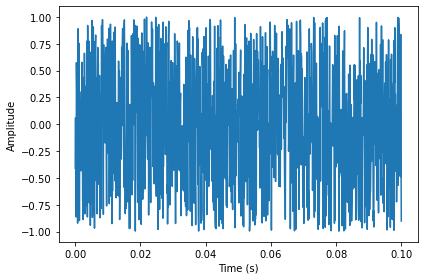
\includegraphics[width=0.75\textwidth]{uun1.png}
		\caption{Сегмент полученного сигнала}
		\label{fig:uun1}
	\end{figure}
	\begin{figure}[H]
		\centering
		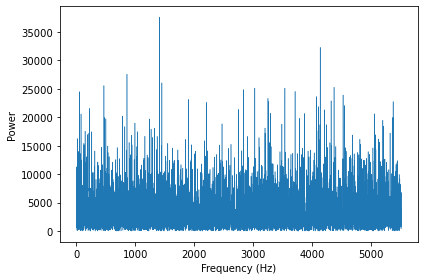
\includegraphics[width=0.75\textwidth]{uun2.png}
		\caption{Спектр энергии сигнала (квадрат амплитуды)}
		\label{fig:uun2}
	\end{figure}
	Некоррелированный шум в среднем имеет одинаковую мощность на всех частотах, что мы можем подтвердить, построив интегральный спектр (нормализованная сумма мощности).
	\begin{lstlisting}[language=Python,caption=Строим интегральный спектр шума]
		integ = spectrum.make_integrated_spectrum()
		integ.plot_power()
	\end{lstlisting}
	\begin{figure}[H]
		\centering
		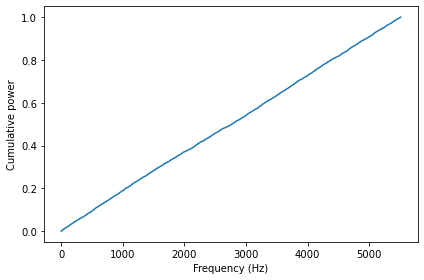
\includegraphics[width=0.75\textwidth]{uun3.png}
		\caption{Результат}
		\label{fig:uun3}
	\end{figure}
	Шум с одинаковой мощностью на всех частотах называется \textquote{Белым} шумом.

	\chapter{Броуновский шум}
	Изучим Броуновский шум.
	\begin{lstlisting}[language=Python,caption=Построение сигнала с Броуновским шумом]
		from thinkdsp import BrownianNoise

		signal = BrownianNoise()
		wave = signal.make_wave(duration = 1, framerate = 11025)
		wave.plot(linewidth = 1)
		spectrum = wave.make_spectrum()
		spectrum.plot_power(linewidth = 0.5)
	\end{lstlisting}
	\begin{figure}[H]
		\centering
		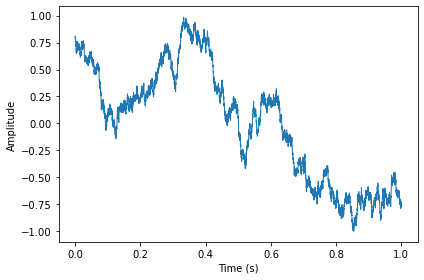
\includegraphics[width=0.75\textwidth]{br1.png}
		\caption{Сигнал с Броуновским шумом}
		\label{fig:br1}
	\end{figure}
	\begin{figure}[H]
		\centering
		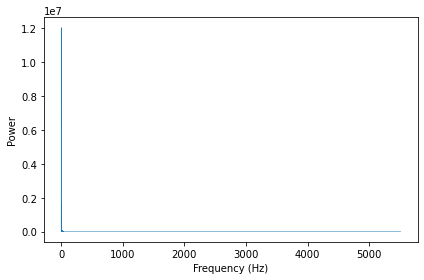
\includegraphics[width=0.75\textwidth]{br2.png}
		\caption{Его зависимость энергии от частоты}
		\label{fig:br2}
	\end{figure}
	Вся энергия сигнала находится на низких частотах. Поэтому, применим логарифмический масштаб.
	\begin{lstlisting}[language=Python,caption=Cигнал с Броуновским шумом в логарифмическом масштабе]
		spectrum.hs[0] = 0
		spectrum.plot_power(linewidth = 0.5)
		loglog = dict(xscale = 'log', yscale = 'log')
		result = spectrum.estimate_slope().slope
	\end{lstlisting}
	\begin{figure}[H]
		\centering
		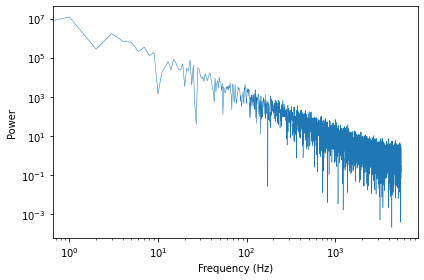
\includegraphics[width=0.75\textwidth]{br3.png}
		\caption{Так лучше видна зависимость энергии сигнала от его частоты}
		\label{fig:br3}
	\end{figure}
	Наклон этой линии приблизительно равен -2, что указывает на зависимость $\frac{1}{f^2}$.

	\chapter{Розовый шум}
	Изучаем \texttt{Розовый шум}. Розовый шум характеризуется параметром $\beta$, обычно между 0 и 2.
	\begin{lstlisting}[language=Python,caption=Построение Розового шума]
		for beta in [0, 1, 2]:
			signal = PinkNoise(beta = beta)
			wave = signal.make_wave(duration=1, framerate=1024)
			spectrum = wave.make_spectrum()
			spectrum.hs[0] = 0
			label = f'beta={beta}'
			spectrum.plot_power(linewidth = 1, alpha = 0.7, label = label)
	\end{lstlisting}
	\begin{figure}[H]
		\centering
		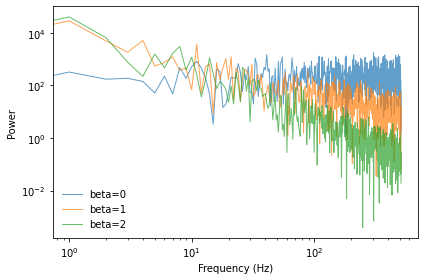
\includegraphics[width=0.75\textwidth]{beta1.png}
		\caption{Результаты построения Розового шума с различным значением аргумента}
		\label{fig:beta1}
	\end{figure}
	При $\beta = 0$ Розовый шум - \textquote{Белый} шум, а при $\beta = 2$ - \textquote{Красный} шум (Броуновский).
	
	\chapter{Гауссов шум}
	А теперь посмотрим на некоррелированный гауссов шум.
	\begin{lstlisting}[language=Python,caption=Гауссов шум]
		from thinkdsp import UncorrelatedGaussianNoise

		signal = UncorrelatedGaussianNoise()
		wave = signal.make_wave(duration=1, framerate=11025)
		wave.plot(linewidth = 0.5)
		spectrum = wave.make_spectrum()
		spectrum.plot_power(linewidth = 1)
	\end{lstlisting}
	\begin{figure}[H]
		\centering
		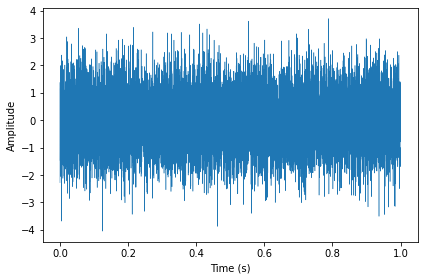
\includegraphics[width=0.75\textwidth]{gaus1.png}
		\caption{Сигнал с гауссовым шумом}
		\label{fig:gaus1}
	\end{figure}
	\begin{figure}[H]
		\centering
		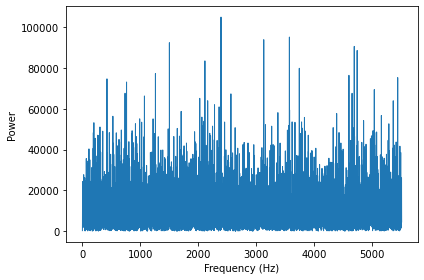
\includegraphics[width=0.75\textwidth]{gaus2.png}
		\caption{Зависимость энергии от частоты}
		\label{fig:gaus2}
	\end{figure}
	\begin{lstlisting}[language=Python,caption=График нормальной вероятности]
		def normal_prob_plot(sample, fit_color = '0.8', **options):
			n = len(sample)
			xs = np.random.normal(0, 1, n)
			xs.sort()
			ys = np.sort(sample)
			mean, std = np.mean(sample), np.std(sample)
			fit_ys = mean + std * xs
			plt.plot(xs, fit_ys, color = 'gray', alpha = 0.5, label = 'model')
			plt.plot(xs, ys, **options)
		
		normal_prob_plot(spectrum.real, color = 'C0', label = 'real part')
		normal_prob_plot(spectrum.imag, color = 'C1', label = 'imag part')
	\end{lstlisting}
	\begin{figure}[H]
		\centering
		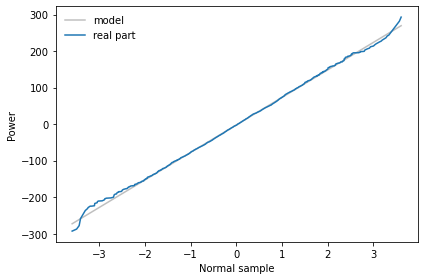
\includegraphics[width=0.75\textwidth]{gaus3.png}
		\caption{Распределение действительной части спектра является гауссовым}
		\label{fig:gaus3}
	\end{figure}
	\begin{figure}[H]
		\centering
		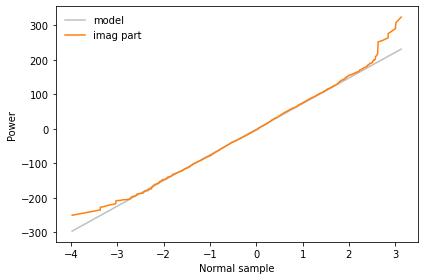
\includegraphics[width=0.75\textwidth]{gaus4.png}
		\caption{Также как и его мнимая часть}
		\label{fig:gaus4}
	\end{figure}

	\chapter{Упражнения}
	\section{Задание 1}
	Исследование природных источнников шума.
	\begin{lstlisting}[language=Python,caption=Два сегмента сигнала с шумом моря]
		from thinkdsp import read_wave

		wave=read_wave('132736__ciccarelli__ocean-waves.wav')
		segment = wave.segment(start = 5.0, duration = 1.0)
		segment2 = wave.segment(start = 10.0, duration = 1.0)
		spectrum = segment.make_spectrum()
		spectrum2 = segment2.make_spectrum()

		spectrum.plot_power(alpha = 0.5)
		spectrum2.plot_power(alpha = 0.5)
		decorate(xlabel = 'Frequency (Hz)', ylabel = 'Amplitude')

		spectrum.plot_power(alpha = 0.5)
		spectrum2.plot_power(alpha = 0.5)
		decorate(xlabel = 'Frequency (Hz)', ylabel = 'Amplitude', **loglog)

		segment.make_spectrogram(512).plot(high = 5000)
	\end{lstlisting}
	\begin{figure}[H]
		\centering
		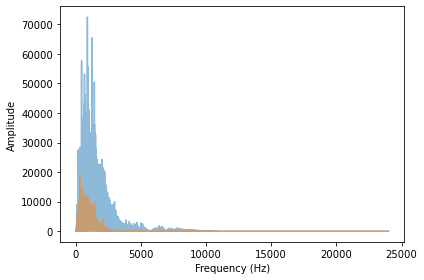
\includegraphics[width=0.75\textwidth]{test1.png}
		\caption{Спектр сигнала}
		\label{fig:test1}
	\end{figure}
	\begin{figure}[H]
		\centering
		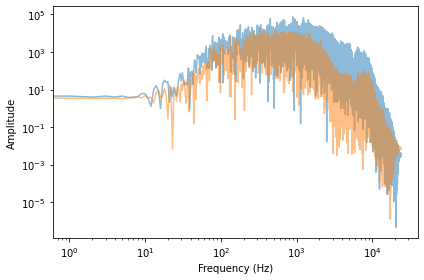
\includegraphics[width=0.75\textwidth]{test2.png}
		\caption{Логарифмический масштаб}
		\label{fig:test2}
	\end{figure}
	\begin{figure}[H]
		\centering
		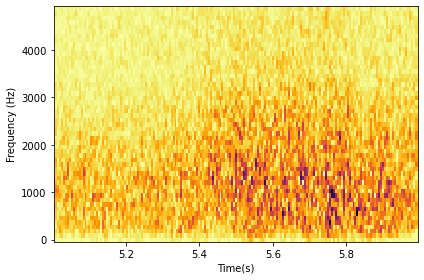
\includegraphics[width=0.75\textwidth]{test3.png}
		\caption{Спектрограмма шума для первого сегмента}
		\label{fig:test3}
	\end{figure}
	Общая амплитуда падает, но смесь частот кажется последовательной.

	\begin{lstlisting}[language=Python,caption=Взяли другой сигнал]
		wave = read_wave('fire.wav')
		segment = wave.segment(start = 1.0, duration = 1.0)
		segment2 = wave.segment(start = 2.5, duration = 1.0)
		...
	\end{lstlisting}
	\begin{figure}[H]
		\centering
		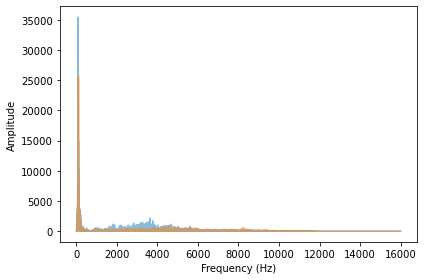
\includegraphics[width=0.75\textwidth]{test4.png}
		\caption{Нашли его спектр}
		\label{fig:test4}
	\end{figure}
	\begin{figure}[H]
		\centering
		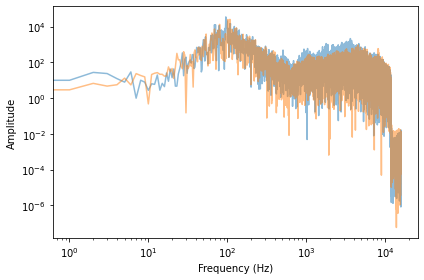
\includegraphics[width=0.75\textwidth]{test5.png}
		\caption{Очень интересная форма}
		\label{fig:test5}
	\end{figure}
	\begin{figure}[H]
		\centering
		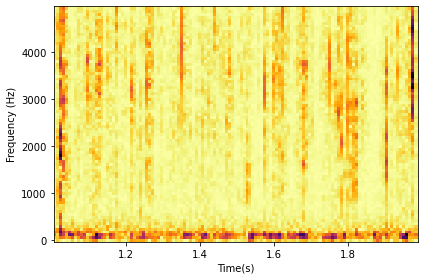
\includegraphics[width=0.75\textwidth]{test6.png}
		\caption{Спектрограмма первого сегмента сигнала}
		\label{fig:test6}
	\end{figure}
	Сигнал чем-то напоминает \textquote{Розовый} шум, но очень отдаленно.
	
	\section{Задание 2}
	Метод Бартлетта и оценка спектра мощности шумового сигнала.
	\begin{lstlisting}[language=Python,caption=Метод Бартлетта]
		from thinkdsp import Spectrum

		def bartlett_method(wave, seg_length = 512, win_flag = True):
			spectro = wave.make_spectrogram(seg_length, win_flag)
			spectrums = spectro.spec_map.values()
			psds = [spectrum.power for spectrum in spectrums]
			hs = np.sqrt(sum(psds) / len(psds))
			fs = next(iter(spectrums)).fs
			spectrum = Spectrum(hs, fs, wave.framerate)
			return spectrum

		psd = bartlett_method(segment)
		psd2 = bartlett_method(segment2)
		psd.plot_power()
		psd2.plot_power()
	\end{lstlisting}
	\begin{figure}[H]
		\centering
		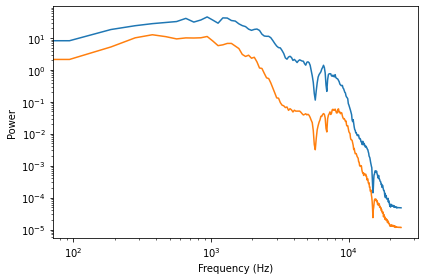
\includegraphics[width=0.75\textwidth]{bartl1.png}
		\caption{Результат применения метода Бартлетта к сигналу шума моря}
		\label{fig:bartl1}
	\end{figure}
	Мы можем более лучше видеть взаимосвязь между мощностью и частотой. Это не простая линейная зависимость, но она последовательна в разных сегментах.	

	\section{Задание 3}
	Спектр цен BitCoin.
	\begin{lstlisting}[language=Python,caption=BitCoin]
		import pandas as pd
		from thinkdsp import Wave

		df = pd.read_csv('BTC_USD_2013-10-01_2020-03-26-CoinDesk.csv', parse_dates=[0])
		ys = df['Closing Price (USD)']
		ts = df.index
		wave = Wave(ys, ts, framerate = 1)
		wave.plot()
		spectrum = wave.make_spectrum()
		spectrum.plot_power()
		spectrum.estimate_slope()[0]
	\end{lstlisting}
	\begin{figure}[H]
		\centering
		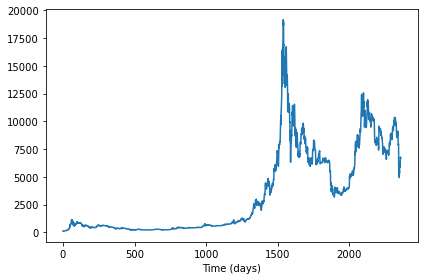
\includegraphics[width=0.75\textwidth]{result1.png}
		\caption{Визуализация изменений цен BitCoin}
		\label{fig:result1}
	\end{figure}
	\begin{figure}[H]
		\centering
		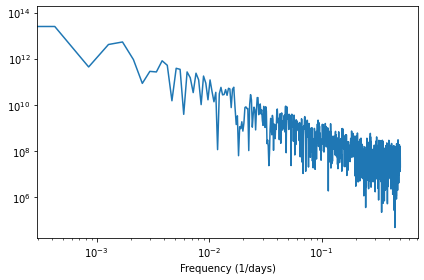
\includegraphics[width=0.75\textwidth]{result2.png}
		\caption{Спектр полученного сигнала в логарифмическом масштабе}
		\label{fig:result2}
	\end{figure}
	Наклон этой кривой близок к 1.7, поэтому трудно сказать, это \textquote{Красный} шум или своего рода \textquote{Розовый} шум.	

	\section{Задание 4}
	Счётчик Гейгера
	\begin{lstlisting}[language=Python,caption=Реализация счётчика Гейгера]
		from thinkdsp import Noise

		class UncorrelatedPoissonNoise(Noise):

			def evaluate(self, ts):
				ys = np.random.poisson(self.amp, len(ts))
				return ys

		amp = 0.001
		framerate = 10000
		duration = 2
		signal = UncorrelatedPoissonNoise(amp = amp)
		wave = signal.make_wave(duration = duration, framerate = framerate)
		expected = amp * framerate * duration
		actual = sum(wave.ys)
		wave.plot()
		spectrum = wave.make_spectrum()
		spectrum.plot_power()
	\end{lstlisting}
	\begin{figure}[H]
		\centering
		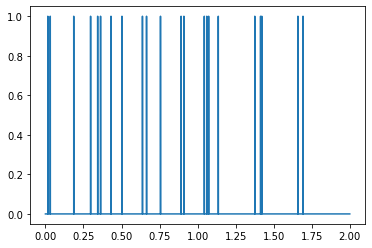
\includegraphics[width=0.75\textwidth]{result3.png}
		\caption{Полученный сигнал}
		\label{fig:result3}
	\end{figure}
	\begin{figure}[H]
		\centering
		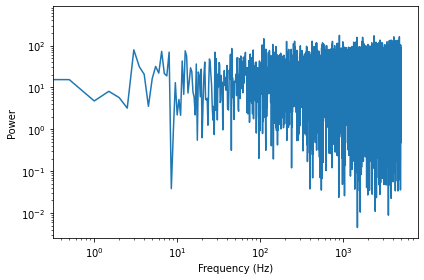
\includegraphics[width=0.75\textwidth]{result4.png}
		\caption{Спектр счетчика Гейгера}
		\label{fig:result4}
	\end{figure}
	Наклон прямой близок к 0, поэтому можно сказать, что это \textquote{Белый} шум.
	\begin{lstlisting}[language=Python,caption=Сравнение спектра с гауссовым шумом]
		amp = 1
		framerate = 10000
		duration = 2
		signal = UncorrelatedPoissonNoise(amp = amp)
		wave = signal.make_wave(duration = duration, framerate = framerate)
		spectrum = wave.make_spectrum()
		spectrum.hs[0] = 0
		normal_prob_plot(spectrum.real, label = 'real')
		normal_prob_plot(spectrum.imag, label = 'imag', color = 'C1')
	\end{lstlisting}
	\begin{figure}[H]
		\centering
		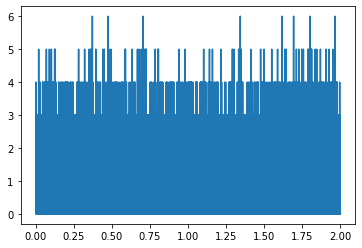
\includegraphics[width=0.75\textwidth]{result5.png}
		\caption{Увеличили амплитуду сигнала}
		\label{fig:result5}
	\end{figure}
	\begin{figure}[H]
		\centering
		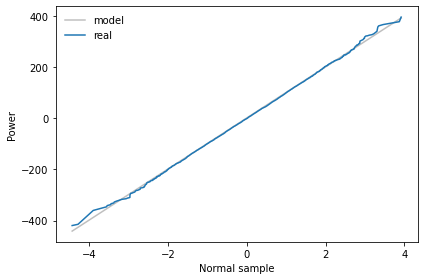
\includegraphics[width=0.75\textwidth]{result6.png}
		\caption{Вещественная часть сигнала}
		\label{fig:result6}
	\end{figure}
	\begin{figure}[H]
		\centering
		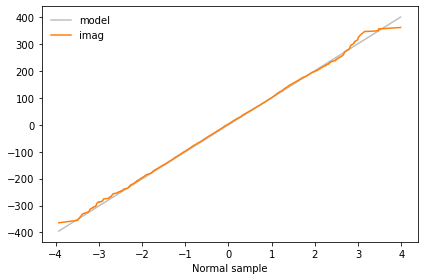
\includegraphics[width=0.75\textwidth]{result7.png}
		\caption{Мнимая часть сигнала}
		\label{fig:result7}
	\end{figure}	

	\section{Задание 5}
	Алгоритм Vocc-McCartney для генерации \textquote{Розового} шума.
	\begin{lstlisting}[language=Python,caption=Итоговая функция]
		def voss(nrows, ncols=16):
			array = np.empty((nrows, ncols))
			array.fill(np.nan)
			array[0, :] = np.random.random(ncols)
			array[:, 0] = np.random.random(nrows)
			n = nrows
			cols = np.random.geometric(0.5, n)
			cols[cols >= ncols] = 0
			rows = np.random.randint(nrows, size = n)
			array[rows, cols] = np.random.random(n)
			df = pd.DataFrame(array)
			df.fillna(method = 'ffill', axis = 0, inplace = True)
			total = df.sum(axis = 1)
			return total.values

		ys = voss(12500)
		wave = Wave(ys)
		wave.plot()
		spectrum = wave.make_spectrum()
		spectrum.hs[0] = 0
		spectrum.plot_power()
	\end{lstlisting}
	\begin{figure}[H]
		\centering
		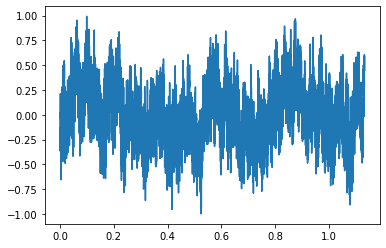
\includegraphics[width=0.75\textwidth]{test7.png}
		\caption{Сигнал, полученный с помощью этой функции}
		\label{fig:test7}
	\end{figure}
	\begin{figure}[H]
		\centering
		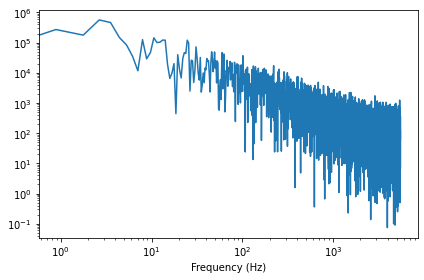
\includegraphics[width=0.75\textwidth]{test8.png}
		\caption{Спектр сигнала в логарифмическом масштабе}
		\label{fig:test8}
	\end{figure}
	Наклон прямой близок к \texttt{-1}.
	\begin{lstlisting}[language=Python,caption=Более длинная выборка]
		seg_length = 64 * 1024
		iters = 100
		wave = Wave(voss(seg_length * iters))
		spectrum = bartlett_method(wave, seg_length = seg_length, win_flag = False)
		spectrum.hs[0] = 0
		spectrum.plot_power()
	\end{lstlisting}
	\begin{figure}[H]
		\centering
		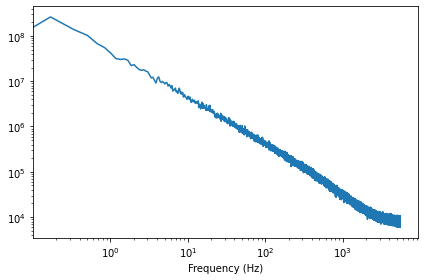
\includegraphics[width=0.75\textwidth]{test9.png}
		\caption{Спектр сигнала с более длинной выборкой в логарифмическом масштабе}
		\label{fig:test9}
	\end{figure}
	Наклон прямой очень близок к \texttt{-1}. Теперь точно можно сказать, что это \textquote{Розовый} шум.

	\chapter{Вывод}
	В данной работе мы познакомились с различными видами шума: \textquote{Белым}, \textquote{Розовым} и \textquote{Красным}. Определили, что их отличает друг от друга. Также рассмотрели спектры некоторых сигналов в логарифмическом масштабе.
\end{document}